% Template for ICASSP-2020 paper; to be used with:
%          spconf.sty  - ICASSP/ICIP LaTeX style file, and
%          IEEEbib.bst - IEEE bibliography style file.
% --------------------------------------------------------------------------
\documentclass{article}
\usepackage{spconf,amsmath,graphicx,xcolor}

% Example definitions.
% --------------------
\def\x{{\mathbf x}}
\def\L{{\cal L}}

\newcommand{\ml}[1]{\textcolor{blue}{ML : #1}}
\newcommand{\fg}[1]{\textcolor{red}{FG : #1}}

% Title.
% ------
\title{Bandwidth extension of musical audio signals with no side information using dilated convolutional neural networks}
%
% Single address.
% ---------------
\name{Mathieu Lagrange, F\'elix Gontier \thanks{Work partially funded by ANR CENSE}}
\address{LS2N, CNRS, Centrale Nantes}
%
% For example:
% ------------
%\address{School\\
%	Department\\
%	Address}
%
% Two addresses (uncomment and modify for two-address case).
% ----------------------------------------------------------
%\twoauthors
%  {A. Author-one, B. Author-two\sthanks{Thanks to XYZ agency for funding.}}
%	{School A-B\\
%	Department A-B\\
%	Address A-B}
%  {C. Author-three, D. Author-four\sthanks{The fourth author performed the work
%	while at ...}}
%	{School C-D\\
%	Department C-D\\
%	Address C-D}
%
\begin{document}
%\ninept
%
\maketitle
%
\begin{abstract}

\end{abstract}
%
\begin{keywords}
Artificial audio bandwidth extension, deep neural network, musical audio processing
\end{keywords}
%
\section{Introduction}
\label{sec:intro}

Bandwidth extension has a long standing history in telecommunication where the bitrate allowed by the given application may be reduced \cite{larsen2005audio}. In this case, it is often beneficial to preserve a good perceptual quality in the lower frequencies, for example to preserve intelligibility for speech applications. In that case, it may interesting to have a processing unit on the receiver that is able to produce a wide-band signal in order to improve perceived quality given the narrow band signal considering the lower frequencies typically up to 4 kHz for speech,.

Many techniques have been introduced, and most of them operates in the spectral domain, where the spectral envelope of the narrow band signal is used to predict the spectral envelope of the higher frequencies. Recent approaches considers deep neural network to do so \cite{abel2017artificial}. This approach assumes a source-filter model for speech production and requires some integration of the two processing units, the one responsible for the narrow band signal decoding and the one responsible for the bandwidth extension. Considering the mapping in the spectral domain using deep neural architecture have been proposed in \cite{li2015deep}. Recurrent neural networks \cite{ling2018waveform} or Wavenet architectures can also be considered \cite{gupta2019speech}. In this case, the network directly predict the wide band speech signal, given some information provided by the conditioning stack that processes the narrow band signal. This approach is very flexible, but computationally demanding.

Due to interoperability requirements in telephony, the bandwidth extension process is done without any side information. That is, the processing unit on the decoder side has to predict the higher frequency signal given some static knowledge and the lower frequency signal only.

In general audio coding, bandwidth extension has been introduced in the beginning of the millennium \cite{dietz2002spectral}. General audio coding is more complex than speech coding due to the variety of physical sources that may produce the signal that has to be encoded. Due to this, and the ability to control the whole transmission stack for most use cases, some side information is considered to perform the bandwidth extension process. This side information is computed using the wide band signal at the encoder side and transmitted within the bitstream. In \cite{dietz2002spectral}, the main concept introduced is called spectral band replication (sbr) where the lower frequencies of the magnitude spectra are duplicated and transposed. Due to the typical exponential decay of magnitude with respect to the frequency, the overall magnitude of the transposed spectra has to be adjusted.

Some post processing steps can be undertaken to further improve the perceptual quality. As the encoder has access to the sbr prediction and the reference high frequency spectra, it is able to adapt to some special cases where considering the high frequency spectrum as the low frequency one will fail. For example,  some high frequency tones that are perceptively salient may not be be recreated using the replication process. In this case, an additional processing unit can be considered to produce salient sinusoidal components \cite{ekstrand2002bandwidth}. The lower frequencies may have strong harmonics and the higher ones only noise like components. In this case, an inverse filtering is applied \cite{ehret2004audio}.

Extension for low delay applications have been proposed \cite{friedrich2007spectral}, as well as the application of the phase vocoder \cite{flanagan1966phase} to reduce unpleasant roughness typically introduced when considering sbr tools \cite{nagel2009harmonic}.

Compared to algorithmic approaches discussed above, considering learning approaches have several benefits. First, if the capacity of the model is sufficient to encode the many relationships between the lower and the higher part of the spectrum and if those encoded relationships are generic enough to produce satisfying results for real use case scenarios, there is no need for side information. Secondly, the relationships encoded by the model being non explicit, there is less chance of reaching a "glass-ceiling" in terms of perceptual quality. Non-negative matrix factorization approaches \cite{sun2013non},  and deep learning approaches have recently been considered \cite{miron2018high}.

To investigate further in this direction, we consider in this paper to consider a deep convolutional network approach that operates in the magnitude spectrum. The model is described in Section \ref{sec:model}. Its performance is evaluated using an experimental protocol described in Section \ref{sec:protocol}. Outcomes of the performance analysis are described in Section \ref{sec:experiments} and discussed in Section \ref{sec:discussion}. \footnote{Reproducible research statement: the experiments described in this paper rely on public data and the code used to produce the results will be made available upon publication.}

\section{Model}
\label{sec:model}

The aim of a bandwidth extension system is to predict the high frequency part. In this paper, we consider audio data represented in the spectral domain. The input and the output of the model consists in 128x10 (frequency x time) matrices that respectively represents the low frequency and high frequency parts of the audio for an approximate duration of $160$ms (more details are provided in Section \ref{sec:protocol}).

The architecture is a fully convolutional neural network \cite{long2015fully} with $L$ layers followed by rectified linear units (ReLU) activations, as described in Figure~\ref{fig:mdl}. The number of output convolution channels $C$ is the same for all hidden layers. Convolution kernels also share the same size $(K_t, K_f)$ in the time and frequency dimensions respectively, and inputs of each layer are padded accordingly so that the size of data representations is held constant throughout the network. Dilated convolutions \cite{yu2016multi, oord2016wavenet} are considered to artificially increase the receptive field of the model, allowing it to capture patterns on larger scales without added parameters. A fixed dilation ratio $D$ is used in the frequency dimension for hidden layers, and no dilation is used in the input and output layers of the network. As a result each hidden layer increases the receptive field by $D(K-1)$ frequency bins compared to $K-1$ without dilation.

\begin{figure}[th]
    \centering
    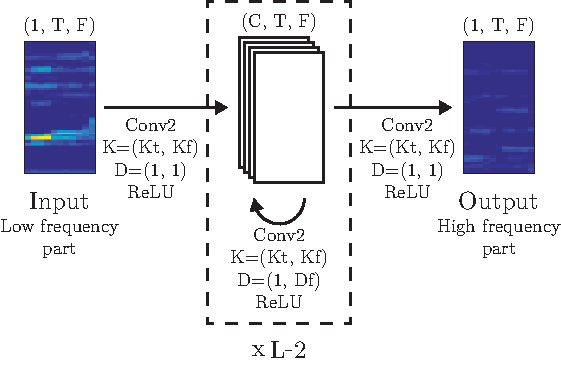
\includegraphics[width=\columnwidth]{figures/mdl.pdf}
    \caption{Proposed deep convolutional neural network architecture for bandwidth extension.}\label{fig:mdl}
\end{figure}

The model is trained using the mean squared error (MSE) loss function of expression:
\begin{equation}
L(y, \hat y) = \frac{1}{N}\sum\limits_{n=1}^{N_b}\sum\limits_{t=1, f=1}^{T, F}(\hat y - y)^2
\end{equation}
where $y$ is the ground truth high frequency part of the spectrum, $\hat y$ is the output of the model, $N_b$ is the batch size, ant $T$ and $F$ are the time and frequency dimensions of the output respectively. Optimization is performed using the Adam \cite{kingma2014adam} algorithm with minibatches of $64$ examples and a learning rate of $0.001$.


\section{Experimental protocol}
\label{sec:protocol}

Two datasets are considered in this study, the \textit{gtzan} dataset \cite{tzanetakis2002musical}, and the \textit{medley-solos-DB} dataset \cite{lostanlen2016deep}. The first comprises 100 polyphonic pop songs of 30 seconds for each of the 10 musical genres represented for a total duration of about 8 hours. The second has 21572 audio clips of about 3 seconds, for a total duration of about 18 hours.

The \textit{gtzan} dataset is split in a training set and testing set using the following procedure. For each genre, the 70 first songs are put in the train set and the 30 remaining in the test set. The \textit{medley-solos-DB} dataset is already split into "training", and "test" datasets, they are considered as is in this study.

For both datasets, the audio data is resampled to $8$kHz and converted to spectral data using a short-term Fourier transform with frame size of $256$ samples, hop size of $128$ samples and a Hann window and split into texture windows of $10$ frames.

The resulting spectra are split into 2 parts, the low frequency one, that serves as input to the different models and the high frequency one serves are reference for training the models and computing the evaluation metrics.

Two metrics are considered. The first metric is the average loss on the test set is used to get a global understanding of the behavior of the predictors in the spectral domain. The second metric is the average signal-to-reconstruction ratio (srr), computed in the time domain. Each batch of texture windows is

Three baselines are considered. The first is a drastically simplified version of the sbr technique, where the high frequency part is simply the low frequency part whose amplitudes are scaled. Please note that this baseline requires some side information, that is the amplitude scaling factor, defined as the ratio of average amplitude between the high frequency part qnd the low frequency one, computed for each texture window.

The second and the third ones are reimplementation of the deep architectures presented in \cite{miron2018high}. The \textit{CNN bottleneck} encoder part consists in two convolutional layers with filters of size $(1, F)$ and $(T, 1)$ that independantly summarize information in the frequency and time dimensions of the input data respectively. A fully connected layer is then applied to extract a code of $64$. The decoder part mirrors these processing steps to recover a spectrum with the original input size. This model is implemented as described in \cite{miron2018high}, though with different filter sizes as $F=128$ and $T=10$ in this study. The \textit{CNN stride-2} autoencoder adopts a different strategy where frequency patterns information is extracted at multiple scales using strided convolutions. The first four layers operate independantly on each time frame, and are followed by two convolutional layers with square kernels. The number of channels increases linearly with each additional layer. In this study, the first two layers are removed to account for the difference in the size of the frequency dimension in considered spectra. For both architectures input examples are logarithmically scaled using the function $log_{10}(1+x)$ to account for the magnitude difference between low and high frequencies, as described by the authors.


\section{Experiments}
\label{sec:experiments}


\begin{figure}
\center
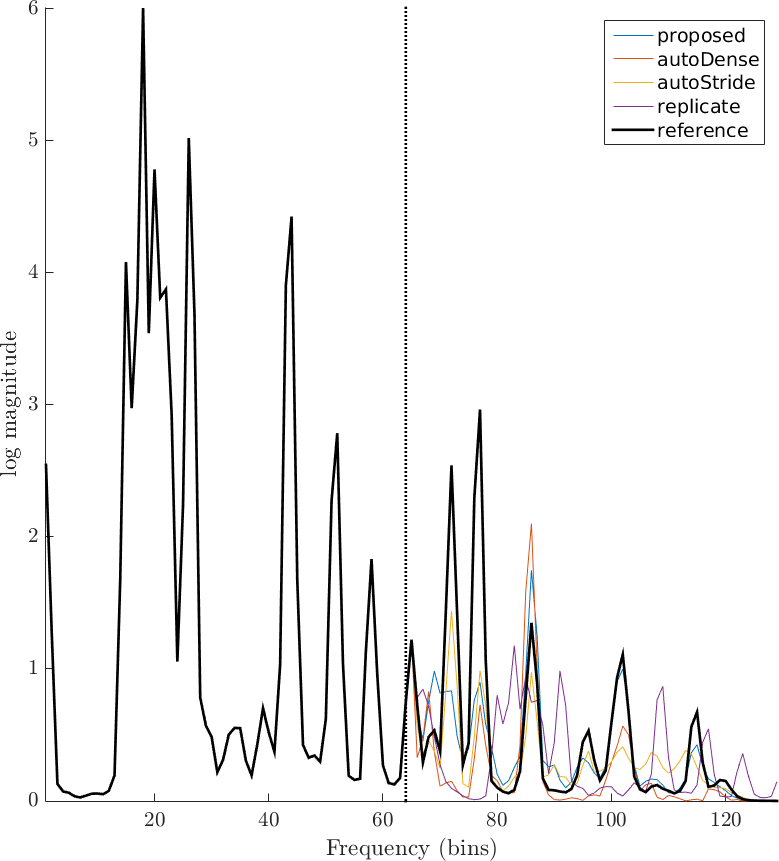
\includegraphics[width = .85\columnwidth]{figures/solos_1141.png}
\caption{Example of spec}
\label{fig:solos}
\end{figure}

\begin{figure}
\center
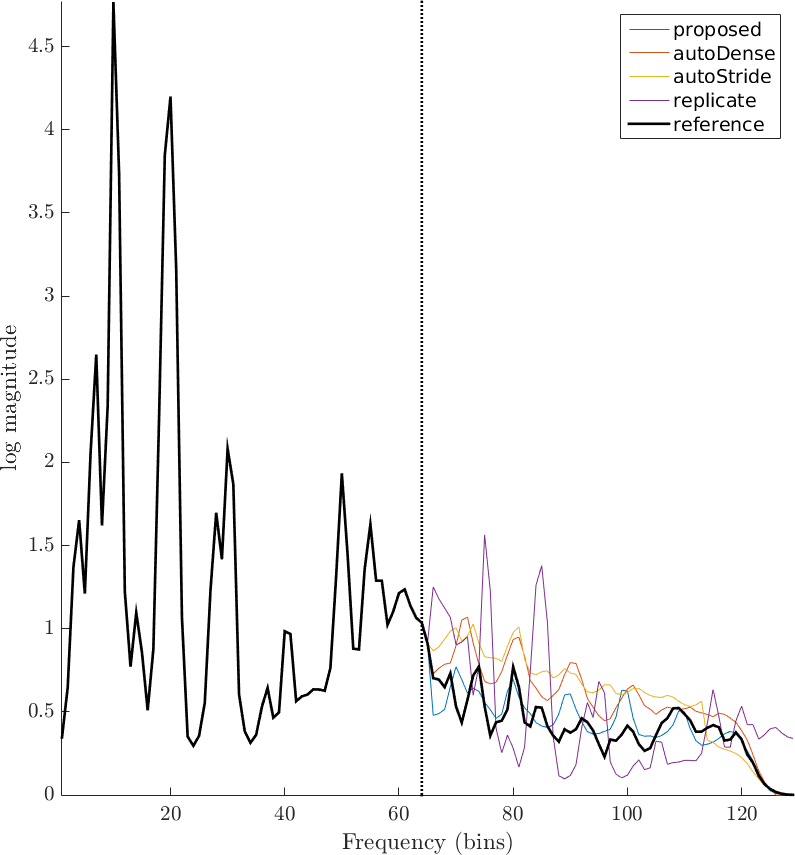
\includegraphics[width = .85\columnwidth]{figures/gtzan_1120.png}
\caption{}
\label{fig:gtzan}
\end{figure}


\begin{table}
\begin{tabular}{llcc}
kernelSize & dilation & gtzan & medleysolos \\
\hline
13 & 1 & 0.109 $\pm$0.020 & 0.237 $\pm$0.014 \\
17 & 1 & 0.105 $\pm$0.021 & 0.226 $\pm$0.016 \\
13 & 2 & 0.102 $\pm$0.021 & 0.226 $\pm$0.017 \\
17 & 2 & 0.102 $\pm$0.022 & 0.218 $\pm$0.019 \\
13 & 3 & - $\pm$- &     - $\pm$- \\
17 & 3 & 0.103 $\pm$0.022 &     - $\pm$- \\
\end{tabular}
\caption{loss kernel size vs dilation}
\end{table}

\begin{table}
\begin{tabular}{llcc}
nbLayers & dilation & gtzan & medleysolos \\
\hline
5 & 1 & 0.110 $\pm$0.017 & 0.240 $\pm$0.013 \\
6 & 1 & 0.107 $\pm$0.021 & 0.231 $\pm$0.016 \\
7 & 1 & 0.105 $\pm$0.021 & 0.226 $\pm$0.016 \\
5 & 2 & 0.102 $\pm$0.019 & 0.228 $\pm$0.015 \\
6 & 2 & 0.102 $\pm$0.022 & 0.225 $\pm$0.019 \\
7 & 2 & 0.102 $\pm$0.022 & 0.218 $\pm$0.019 \\
5 & 3 & - $\pm$- &     - $\pm$- \\
6 & 3 & - $\pm$- &     - $\pm$- \\
7 & 3 & 0.103 $\pm$0.022 &     - $\pm$- \\
\end{tabular}
\caption{loss layers vs dilation}
\end{table}

\begin{table}
\begin{tabular}{llcc}
nbChannels & dilation & gtzan & medleysolos \\
\hline
 32 & 1 & 0.108 $\pm$0.020 & 0.237 $\pm$0.014 \\
 64 & 1 & 0.107 $\pm$0.021 & 0.231 $\pm$0.016 \\
128 & 1 & 0.107 $\pm$0.019 & 0.233 $\pm$0.014 \\
 32 & 2 & 0.102 $\pm$0.021 & 0.229 $\pm$0.016 \\
 64 & 2 & 0.102 $\pm$0.022 & 0.225 $\pm$0.019 \\
128 & 2 & 0.101 $\pm$0.020 & 0.220 $\pm$0.017 \\
\end{tabular}
\caption{loss channels vs dilation}
\end{table}

\begin{table}
\begin{tabular}{lcc}
method & gtzan & medleysolos \\
\hline
dnn & 0.102 $\pm$0.022 & 0.225 $\pm$0.019 \\
autoDense & 0.107 $\pm$0.017 & 0.241 $\pm$0.011 \\
autoStride & 0.110 $\pm$0.017 & 0.228 $\pm$0.013 \\
\end{tabular}
\caption{loss proposed 17 6 64 vs soa}
\end{table}


\begin{table}
  \begin{tabular}{lcc}
  method   & mirror & oracle \\
  \hline
  null & 12.91 $\pm$3.26 &  12.91 $\pm$3.26 \\
  replicate & 10.84 $\pm$3.30 & 13.30 $\pm$3.22 \\
\hline
  autoDense & 11.14 $\pm$2.98 & 15.62 $\pm$3.23 \\
  autoStride & 11.20 $\pm$2.84 & 15.58 $\pm$3.10 \\
  \hline
  proposed  & 11.28 $\pm$2.98 & 16.32 $\pm$3.31\\
  \hline
  oracle & 10.51 $\pm$3.26 & $\infty$ \\
  \end{tabular}
  \caption{gtzan srr}
\end{table}

\begin{table}
\begin{tabular}{lcc}
method & mirror & oracle \\
\hline
null & 12.93 $\pm$3.11 & 12.93 $\pm$3.11\\
replicate & 10.70 $\pm$2.90 & 11.61 $\pm$2.88\\
\hline
autoDense & 10.59 $\pm$2.54 &  13.26 $\pm$2.77\\
autoStride & 11.23 $\pm$2.58 & 13.86 $\pm$2.69 \\
\hline
proposed  & 10.99 $\pm$2.44 & 14.29 $\pm$2.60 \\
\hline
oracle & 10.50 $\pm$3.12 & $\infty$ \\
\end{tabular}
\caption{solos srr}
\end{table}




\section{Discussion}
\label{sec:discussion}

X Y

good performance analysis properties

extension on generalization studies

potential creative usage

\vfill\pagebreak


\bibliographystyle{IEEEbib}
\bibliography{strings,refs}

\end{document}
